\documentclass[1p]{elsarticle}

\usepackage[english]{babel}
\usepackage[utf8]{inputenc}
\usepackage[T1]{fontenc}
\usepackage{amsmath}
\usepackage{amssymb}
\usepackage{bm}
\usepackage{xcolor}
\usepackage{algpseudocode}
\usepackage{graphicx}
\usepackage{subfigure}
\usepackage{hyperref}
\usepackage{cleveref}

\bibliographystyle{elsarticle-num}
\journal{Physica A: Statistical Mechanics and its Applications}

\begin{document}

\author[Smith]{Vasily~Postnicov}
\author[Smith]{Marina~V.~Karsanina}
\author[Smith,MIT]{Aleksey~Khlyupin}
\author[Smith]{Kirill~M.~Gerke\corref{maincorr}}
\cortext[maincorr]{Corresponding author}
\ead{kg@ifz.ru}

\address[Smith]{Schmidt Institute of Physics of the Earth of Russian Academy of
  Sciences, Moscow, 107031, Russia}
\address[MIT]{Moscow Institute of Physics and Technology,
  Dolgoprudny, 141701, Russia}
%\affiliation{\textsuperscript{3}Oil and Gas Research Institute Russian Academy
%  of Sciences (OGRI RAS) 3, Gubkina st., Moscow, 119333, Russian Federation}

\title{Another paper with lots of text and fancy pictures}

\begin{abstract}
  Wow, we can multiply arrays and tell you how cool it is.
\end{abstract}

\begin{keyword}
  Arrays, multiplication, addition
\end{keyword}

\maketitle

\section{Theoretical background}
Let $A_1, A_2, \dots, A_n$ be pairwise disjoint subsets of a set
$A \subset \mathbb{R}^n$. We introduce a family of indicator functions
$I_n(x) : A \rightarrow \{0,1\}$ defined as:
\begin{equation}
  I_n(x) = \left\{
  \begin{array}{ll}
    1 & \quad x \in A \\
    0 & \quad \text{otherwise}
  \end{array}
  \right.
\end{equation}

Now we can define the three-point correlation function $S_3: A^2 \rightarrow [0, 1]$:
\begin{equation}
  S_3^n(x_1, x_2) = \langle I_n(x) I_n(x + x_1) I_n(x + x_2) \rangle
\end{equation}
It can be understood as the probability that all three vertices of a triangle
$(0, x_1, x_2)$ will appear in the subset $A_n$ when it is randomly thrown in
$A$. When $A$ represent isotropic medium, $x_1$ and $x_2$ can be replaced with
three numbers $r_1 = |x_1|$, $r_2 = |x_2|$ and $r_3 = |x_2 - x_1|$ to get a
function $S_3: [0, \infty)^3 \rightarrow [0, 1]$.

Another function closely related to the three-point correlation function is the
cluster function which can be defined as
\begin{equation}
  C_3^n(x_1, x_2) = \sum_{k=1}^K \langle \tilde{I}_k(x) \tilde{I}_k(x + x_1) \tilde{I}_k(x + x_2) \rangle
\end{equation}
where $\tilde{I}_k$ is an indicator function for $k$-th cluster and $K$ is a
total number of clusters. A cluster is a subset of $A_n$ so that any two points
in this subset can be connected with a curve belonging to that subset.

Introduce a function $M_n(x) = |\nabla I_n(x)|$ which is a so-called interface
indicator function. With this function we can define three additional
correlation functions, which are the surface-surface-surface function
($F_{sss}$), surface-surface-void function ($F_{ssv}$) and surface-void-void
function ($F_{svv}$). They are defined as
\begin{align}
  F_{sss}^n(x_1, x_2) &= \langle M_n(x) M_n(x + x_1) M_n(x + x_2) \rangle \\
  F_{ssv}^n(x_1, x_2) &= \langle M_n(x) M_v(x + x_1) I_v(x + x_2) \rangle \\
  F_{svv}^n(x_1, x_2) &= \langle M_n(x) I_v(x + x_1) I_v(x + x_2) \rangle
\end{align}
Here $I_v$ is an indicator function for the subset of the void phase
$A_v$. Unlike $S_3$ and $C_3$ functions, these functions do not have the meaning
of probability and have the units of measurement inversely proportional to
volume, surface and length, respectively (e.g. $\mu m^{-3}$, $\mu m^{-2}$ and
$\mu m^{-1}$). These functions describe the interface of the subset $A_n$ and
its spatial configuration with respect to $A_v$.

\section{Computational algorithms}
Three-point correlation function $S_3$ can be computed either in spatial domain
or in frequency domain via the convolution theorem. The simplest algorithm below
calculates $S_3$ pointwise in spatial domain:
\begin{algorithmic}[1]
  \Procedure{$S_3$}{$A, n, x_1, x_2$}
  \State $A_n \gets I_n (A)$
  \State $A'_n \gets \mathfrak{S}(A_n, x_1)$
  \State $A''_n \gets \mathfrak{S}(A_n, x_2)$
  \State $T \gets A_n \cdot A'_n \cdot A''_n$
  \State \textbf{return} $Sum(T) / Norm(A, x_1, x_2)$
  \EndProcedure
\end{algorithmic}
In this algorithm the indicator function $I_n$ for the phase of interest $n$ is
applied to the input array $A$. Then the shift operator $\mathfrak{S}$ is used
to shift $A_n$ by vectors $x_1$ and $x_2$. Finally, the three arrays are
multiplied pointwise and normalized sum of all elements of the product is
returned.

There are two common boundary conditions when applying $\mathfrak{S}$. The first
condition is to extend $A_n$ periodically (\cref{fig:s3-periodic}) when
accessing out-of-bounds array elements. This is the same as circular-shifting
$A_n$. In this case $Norm(A, x_1, x_2)$ does not depend on $x_1$ and $x_2$ and
is equal to the total number of elements in $A$. The second condition is to
replace out-of-bound elements with zeros (so-called zero padding)
(\cref{fig:s3-zeros}). A formula for $Norm(A, x_1, x_2)$ in this case is in
\ref{sec:number-of-trials}.
\begin{figure*}[tp]
  \centering
  \subfigure[Periodic boundary conditions]{
    \includegraphics[width=0.45\linewidth]{images/periodic.png}
    \label{fig:s3-periodic}}
  \hfill
  \subfigure[Zero padding]{
    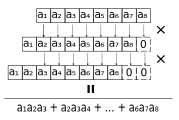
\includegraphics[width=0.45\linewidth]{images/zeros.png}
    \label{fig:s3-zeros}}
  \caption[]{Computation of unnormalized $S_3$ function at point $(1, 2)$ for
    one-dimensional sequence of length 8.}
  \label{fig:s3-computation}
\end{figure*}

The second approach is to compute the whole correlation map in Fourier
domain. Suppose we have a function
$f: \mathbb{R} \rightarrow \mathbb{R}$. Triple correlation for this function is
a function
\begin{equation}
  g(t_1, t_2) = \int f(\tau) f(\tau + t_1) f(\tau + t_2) d \tau
\end{equation}
We can use a well-known formula to compute Fourier image of $g$:
\begin{equation}
  \hat{g}(z_1, z_2) = \hat{f}(z_1) \hat{f}(z_2) \overline{\hat{f}(z_1 + z_2)}
\end{equation}
This algorithm has a better computational complexity compared with the previous
algorithms if the whole correlation map is needed ($O(n \log n)$ vs
$O(n^2)$). The whole correlation map, however, requires a lot of memory and is
rarely needed. Imagine, that the input array $A$ is of dimensions
$500 \times 500$. Then, considering that single precision floating point numbers
are used, $4 \cdot 2 \cdot 500^4 / 1000^3 = 500$ GB are needed to store Fourier
image of the map. Moreover, Fourier image of the whole map is needed even if
only one element of the map in spatial domain is required. The aforementioned
limitations render this approach very impractical.

Our implementation fixes $x_1$ and $x_2$ to be parallel to one of the axes $X$,
$Y$ or $Z$ with restriction $x_1 \perp x_2$ (\cref{fig:pattern}). Thus, the
output has dimensions $D_1 \times D_2$ where $D_1$ and $D_2$ are dimensions of
the input array along selected axes.
\begin{figure}[ht]
  \centering
  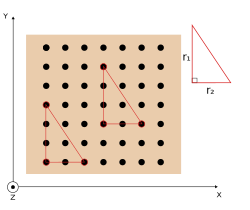
\includegraphics[width=0.5\linewidth]{images/pattern.png}
  \caption[]{Pattern used for calculation of $S_3$ function in out
    implementation. Vectors $x_1$ and $x_2$ are parallel to one of the axes $X$,
    $Y$ or $Z$ and have lengths $r_1$ and $r_2$ respectively.}
  \label{fig:pattern}
\end{figure}

Algorithms for three-point surface functions are the same as for $S_3$,
containing only small modifications. The main difference is that we need to
replace an indicator function $I_n$ with an edge detection operator $E_n$
(see \ref{sec:filter}). Then the algorithms are straightforward:
\begin{algorithmic}[1]
  \Procedure{$F_{sss}$}{$A, n, x_1, x_2$}
  \State $A_n \gets E_n (A)$
  \State $A'_n \gets \mathfrak{S}(A_n, x_1)$
  \State $A''_n \gets \mathfrak{S}(A_n, x_2)$
  \State $T \gets A_n \cdot A'_n \cdot A''_n$
  \State \textbf{return} $Sum(T) / Norm(A, x_1, x_2)$
  \EndProcedure

  \Procedure{$F_{ssv}$}{$A, n, x_1, x_2$}
  \State $A_n \gets E_n (A)$
  \State $A_{(void)} \gets I_{(void)} (A)$
  \State $A'_n \gets \mathfrak{S}(A_n, x_1)$
  \State $A'_{(void)} \gets \mathfrak{S}(A_{(void)}, x_2)$
  \State $T \gets A_n \cdot A'_n \cdot A'_{(void)}$
  \State \textbf{return} $Sum(T) / Norm(A, x_1, x_2)$
  \EndProcedure

  \Procedure{$F_{svv}$}{$A, n, x_1, x_2$}
  \State $A_n \gets E_n (A)$
  \State $A_{(void)} \gets I_{(void)} (A)$
  \State $A'_{(void)} \gets \mathfrak{S}(A_{(void)}, x_1)$
  \State $A''_{(void)} \gets \mathfrak{S}(A_{(void)}, x_2)$
  \State $T \gets A_n \cdot A'_{(void)} \cdot A''_{(void)}$
  \State \textbf{return} $Sum(T) / Norm(A, x_1, x_2)$
  \EndProcedure
\end{algorithmic}

To compute $C_3$ function we need to use a connected-component labeling
algorithm \cite{4728561,PhysRevB.14.3438} to label clusters. Then, again, a
slightly modified algorithm for $S_3$ is used.
\begin{algorithmic}[1]
  \Procedure{$C_3$}{$A, n, x_1, x_2$}
  \State $A_n \gets I_n (A)$
  \State $C_n \gets \mathfrak{C}(A_n)$
  \State $C'_n \gets \mathfrak{S}(C_n, x_1)$
  \State $C''_n \gets \mathfrak{S}(C_n, x_2)$
  \State $T \gets C_n \odot C'_n \odot C''_n$
  \State \textbf{return} $Sum(T) / Norm(A, x_1, x_2)$
  \EndProcedure
\end{algorithmic}
Here $\mathfrak{C}$ is connected-component labeling operator and $\odot$ is
defined as follows:
\begin{equation}
  x \odot y = \left\{
  \begin{array}{ll}
    1 & \quad x = y \\
    0 & \quad \text{otherwise}
  \end{array}
  \right.
\end{equation}

\section{Verification}
To verify correctness of computation of $S_3$ and $C_3$ functions we use the
following simple relations:
\begin{align}
  & S_3^n (x, 0) = S_3^n (0, x) = S_2^n(x) \\
  & C_3^n (x, 0) = C_3^n (0, x) = C_2^n(x) \\
  & \lim_{\substack{x_1 \to \infty \\ x_2 \to \infty}} S_3^n (x_1, x_2) =
  \lim_{\substack{x_1 \to \infty \\ x_2 \to \infty}} C_3^n (x_1, x_2) = \phi_n^3
\end{align}
Here $\phi_n$ is a fraction of phase $n$ in $A$.

There are only few sets for which analytic expressions for $S_2$ are known. One
of those is a set consisting of overlapping balls with a fixed radius $R$ and
centers generated with Poisson process with parameter $\lambda$. In this case
the expression for $S_2$ is following:
\begin{equation}
  \begin{aligned}
    S_2(r, R) &= \exp(-\frac{4}{3}\pi\lambda R^3 f(r, R)) \\
    f(r, R) &= \left\{
    \begin{array}{ll}
      1 + \frac{3}{4} \frac{r}{R} - \frac{1}{16} (\frac{r}{R})^3 & \quad r < 2R \\
      2 & \quad \text{otherwise}
    \end{array}
    \right.
  \end{aligned}
  \label{eq:s2-balls}
\end{equation}

On \cref{fig:balls} there is an intersection of such a set with $R = 0.02$ and
$\lambda=5000$ and a cube $[0, 1]^3$. Because $R \ll 1$, we can use
\cref{eq:s2-balls} to verify our computations what we do on
\cref{fig:balls-s3-comparison}.
\begin{figure*}[tp]
  \centering
  \subfigure[Realization of overlapping balls]{
    \includegraphics[width=0.45\linewidth]{images/balls.png}
    \label{fig:balls}}
  \hfill
  \subfigure[A plot of $S_3(0, r)$ computed with our algorithm and theoretical
    formula.]{
    \includegraphics[width=0.45\linewidth]{images/balls-s3.png}
    \label{fig:balls-s3-comparison}}
  \caption[]{A comparison of calculated and theoretical values of $S_3$ function
    for overlapping balls.}
  \label{fig:s3-verification}
\end{figure*}

\textcolor{red}{What about $C_3$?}

To test $F_{sss}$ function we use a recently developed approach which computes
that function for sets defined by inequation $f(x) \le T$, $x \in \mathbb{R}^3$
with help of automatic differentiation \cite{postnicov20232}. We choose $f$
\begin{equation}
  f(x, y, z) = \sqrt{x^2 + y^2 + z^2}
\end{equation}
so inequation $f(x, y, z) \le T$ gives us a ball.

The test was performed by evaluating the inequation with the parameter $T = 0.2$
in a cube $[0, 1]^3$ and comparing $F_{sss}$ calculated with our algorithm with
precise values. The result of comparison is on
\cref{fig:sss-verification}. Maximal relative error for this case is about  15\%
when $F_{sss}(r_1, r_2)$ is calculated for $r_1$ and $r_2$ being not too close
to zero.
\begin{figure*}[tp]
  \centering
  \subfigure[Computation with our algorithm]{
    \includegraphics[width=0.45\linewidth]{images/ball-sss.png}
    \label{fig:balls-sss-comp}}
  \hfill
  \subfigure[Relative error of computation]{
    \includegraphics[width=0.45\linewidth]{images/ball-sss-error.png}
    \label{fig:ball-sss-error}}
  \caption[]{Comparison of $F_{sss}$ function for a ball with the radius $0.2$
    with precise values.}
  \label{fig:sss-verification}
\end{figure*}

To test $F_{ssv}$ and $F_{svv}$ we use the following relations for such a set
$A$ where all non-void phase is covered by a ball $\mathfrak{O}(R)$:
\begin{align}
  F^n_{ssv}(x_1, x_2) &= F^n_{ss}(x_1) \qquad x_2 > R \\
  F^n_{svv}(x_1, x_2) &= F^n_{sv}(x_1) \qquad x_2 > R
\end{align}
$F_{ss}$ and $F_{sv}$ functions are well-known for a ball of radius $R$ (solid
phase) placed in the center of cube of volume $V$ (void phase):
\begin{align}
  F_{ss}(r, R) &= \frac{1}{V} \left\{
    \begin{array}{ll}
      2\pi R^2/r & \quad r < 2R \\
      0 & \quad \text{otherwise}
    \end{array}
    \right.\\
  F_{sv}(r, R) &= \frac{1}{V} \left\{
    \begin{array}{ll}
      \pi Rr + 2\pi R^2 & \quad r < 2R \\
      4\pi R^2 & \quad \text{otherwise}
    \end{array}
    \right.
\end{align}
The comparison of our algorithm against theory is on
\cref{fig:surface-verification}. Radius of the ball is chosen $R=0.2$.
\begin{figure*}[tp]
  \centering
  \subfigure[$F_{ssv}$]{
    \includegraphics[width=0.45\linewidth]{images/ball-ssv.png}
    \label{fig:balls-ssv}}
  \hfill
  \subfigure[$F_{svv}$]{
    \includegraphics[width=0.45\linewidth]{images/ball-svv.png}
    \label{fig:ball-svv}}
  \caption[]{Comparison of $F_{ssv}$ and $F_{svv}$ functions for a ball with the
    radius $0.2$ with theoretical values.}
  \label{fig:surface-verification}
\end{figure*}


\section{Results}
In this section we compute correlation functions for some real samples. Table
\ref{tab:summary} contains information about these samples.
\begin{table}[!htp]
  \centering
  \begin{tabular}{|c|c|c|c|c|}
    \hline
    Sample name & Image type & Dimensions (pixels) & Image resolution ($\mu m$) & $C_{0.5}$\\
    \hline
    Ceramic 1   & XCT & $500 \times 500 \times 500$ & 2.25 & 0.9823 \\
    Ceramic 2   & XCT & $500 \times 500 \times 500$ & 2.25 & 0.9890 \\
    Ceramic 3   & XCT & $500 \times 500 \times 500$ & 2.25 & 0.9712 \\
    Sandstone 1 & SEM &  $1280 \times 869$ & 0.10 & 0.9703 \\
    Sandstone 2 & SEM &  $1280 \times 869$ & 0.05 & 0.9897 \\
    Carbonate 1 & SEM &  $1024 \times 691$ & 0.06 & 0.9721 \\
    \hline
  \end{tabular}
  \caption{Summary of samples used for calculation of correlation functions.}
  \label{tab:summary}
\end{table}


\section{Discussion}
In this paper we have provided two approaches to compute three-point correlation
function:
\begin{enumerate}
\item Computation in frequency domain using Fourier transform. This approach has
  computational complexity $O(n \log n)$ and computes the whole correlation
  map. Unfortunately, it requires $O(n^2)$ additional memory and therefore can
  be used only with small inputs. Moreover, the whole Fourier image of the input
  is needed even if we need only a small part of the correlation map.
\item Computation in spatial domain. This approach is implemented by us in
  CorrelationFunctions.jl package. This approach calculates the full map with
  complexity $O(n^2)$ but uses only $O(n)$ additional memory for shifted
  versions of the input. For our purposes the whole map is not needed and
  therefore the amount of calculations can be significantly reduced.
\end{enumerate}
It's tempting to create an algorithm which unites advantages of both approaches
(fast speed of the first and low memory consumption of the second) which
computes some desired slices of correlation map. It is known that Fourier
transform is the only linear transform which allows computation of convolution
in $O(n)$. It is still an open question if there are linear transforms which
allow computation of convolution with complexity between $O(n)$ and $O(n^2)$
\cite{stone2008uniqueness,stone1998convolution}.

\appendix
\section{Computation of number of trials for non-periodic mode}
\label{sec:number-of-trials}
If the displacement vectors $x_1, x_2: x_1 \perp x_2$ are parallel to two
distinct unit vectors $i=(1,0,0)$, $j=(0,1,0)$ or $k=(0,0,1)$ then the number of
trials for the input array having dimensions $D = (D_x, D_y, D_z)$ is the
following:
\begin{equation}
  \begin{aligned}
    & Norm(A, x_1, x_2) = \prod_k D'_k \\
    & D' = D - x_1 - x_2
  \end{aligned}
\end{equation}

\section{Edge detection filter}
\label{sec:filter}
For edge detection we use a kernel with the width 7 with coefficients inversely
proportional to distance to kernel's central element. The central element has
such value, so all elements of the kernel sum to zero:
\begin{equation}
  E_k = S \left\{
  \begin{array}{ll}
    -\sum\limits_{\substack{l \\ l \ne 0}} E_l & \quad k = 0 \\
    1 / \rho(k, 0) & \quad \text{otherwise}
  \end{array}
  \right.
\end{equation}
For 3D case $S=172.96$ and for 2D case $S=30.46$.

\bibliography{paper}
\end{document}
